\RequirePackage{luatex85}
\documentclass[tikz, border=10pt]{standalone}

\usepackage[compat=1.1.0]{tikz-feynman}

\begin{document}

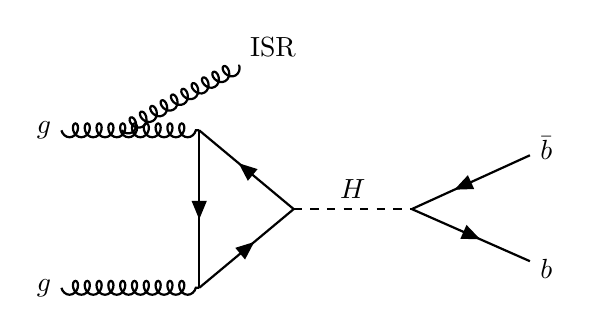
\begin{tikzpicture}[thick]
 \begin{feynman}
  \vertex (origin);
  \vertex [right=1.5cm of origin] (H);
  \vertex [above right=0.50cm and 1.5cm of H] (b1) {\(\bar{b}\)};
  \vertex [below right=0.50cm and 1.5cm of H] (b2) {\(b\)};
  \vertex [above left=1cm and 1.2cm of origin] (v1);
  \vertex [below left=1cm and 1.2cm of origin] (v2);
  \vertex [left=1.75cm of v1] (g1) {\(g\)};
  \vertex [left=1.75cm of v2] (g2) {\(g\)};
  \vertex at ($(g1)!0.5!(v1)$) (ISR_start);
  \vertex [above right=0.8cm and 1.5 cm of ISR_start] (ISR) {ISR};
  \diagram* {
  (origin) -- [scalar, edge label={\(H\)}] (H) -- [anti fermion] (b1),
  (H) -- [fermion] (b2),
  (origin) -- [fermion] (v1) -- [fermion] (v2) -- [fermion] (origin),
  (g1) -- [gluon] (v1),
  (g2) -- [gluon] (v2),
  (ISR_start) -- [gluon] (ISR),
  };
 \end{feynman}
\end{tikzpicture}
\end{document}
